% Created by tikzDevice version 0.12.6 on 2026-08-11 03:14:40
% !TEX encoding = UTF-8 Unicode
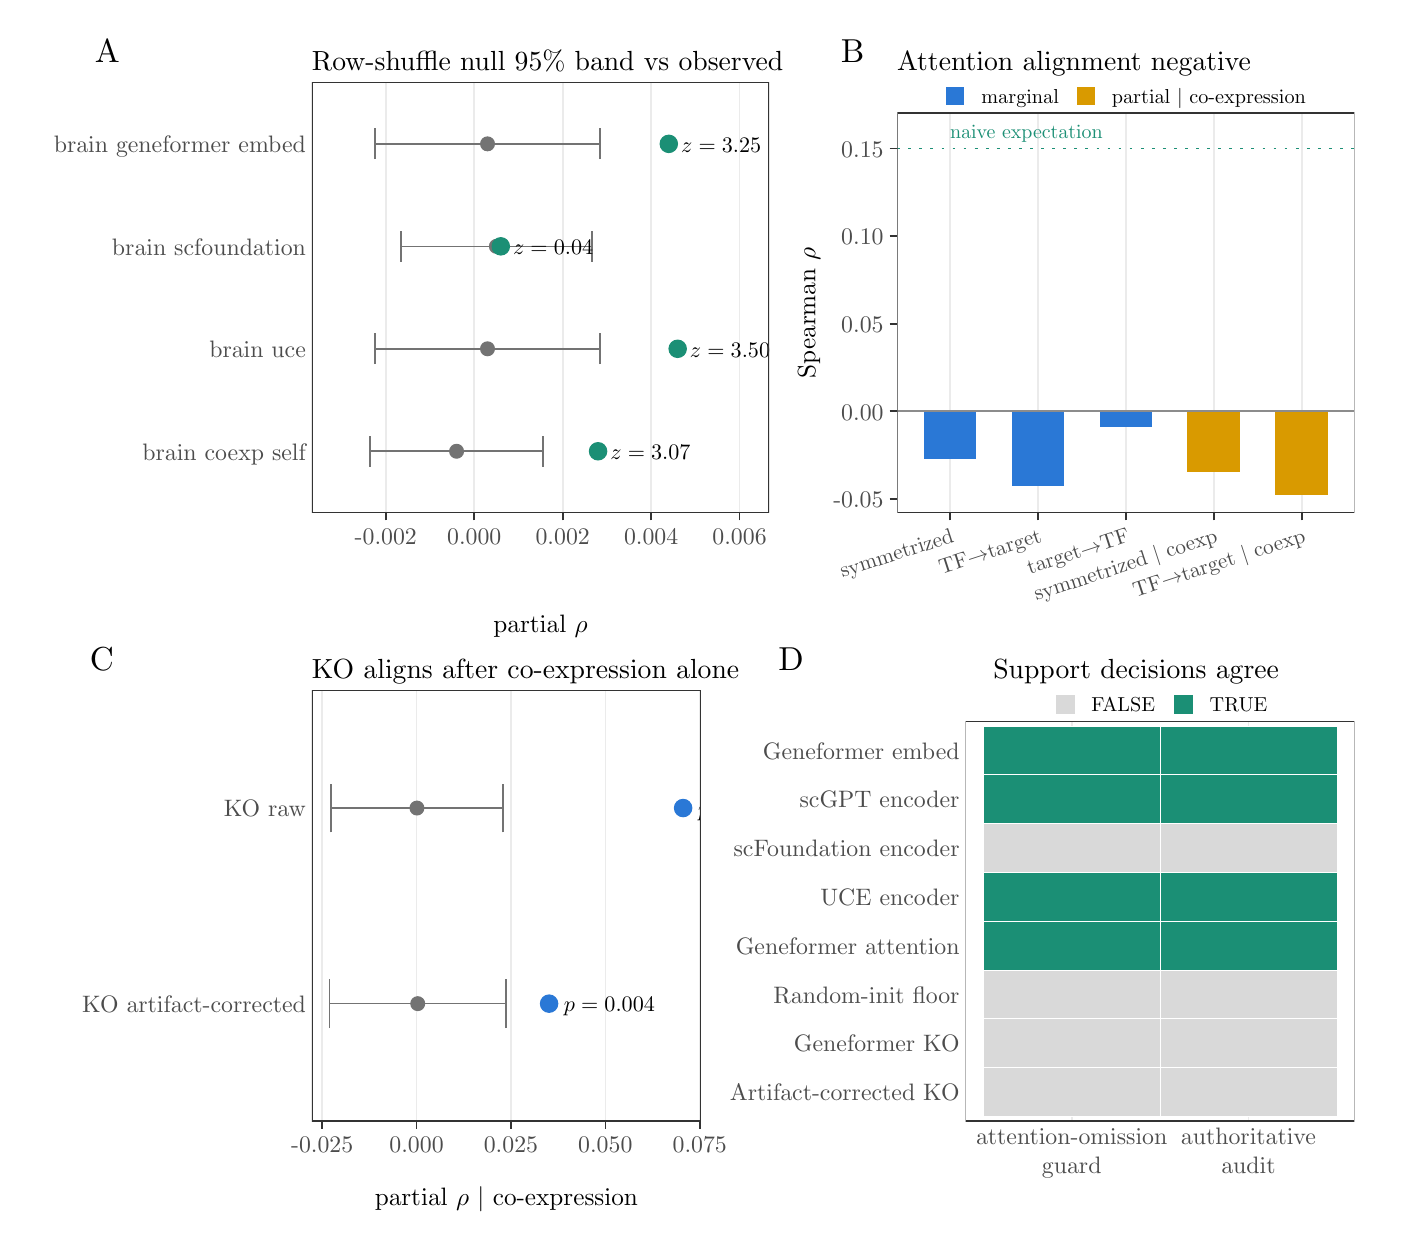
\begin{tikzpicture}[x=1pt,y=1pt]
\definecolor{fillColor}{RGB}{255,255,255}
\path[use as bounding box,fill=fillColor,fill opacity=0.00] (0,0) rectangle (491.44,433.62);
\begin{scope}
\path[clip] (  0.00,  0.00) rectangle (491.44,433.62);
\definecolor{drawColor}{RGB}{255,255,255}
\definecolor{fillColor}{RGB}{255,255,255}

\path[draw=drawColor,line width= 0.6pt,line join=round,line cap=round,fill=fillColor] (  0.00,  0.00) rectangle (491.44,433.62);
\end{scope}
\begin{scope}
\path[clip] (  4.00,209.82) rectangle (273.94,429.62);
\definecolor{drawColor}{RGB}{255,255,255}
\definecolor{fillColor}{RGB}{255,255,255}

\path[draw=drawColor,line width= 0.6pt,line join=round,line cap=round,fill=fillColor] (  4.00,209.82) rectangle (273.94,429.62);
\end{scope}
\begin{scope}
\path[clip] (273.94,209.82) rectangle (485.44,429.62);
\definecolor{drawColor}{RGB}{255,255,255}
\definecolor{fillColor}{RGB}{255,255,255}

\path[draw=drawColor,line width= 0.6pt,line join=round,line cap=round,fill=fillColor] (273.94,209.82) rectangle (485.44,429.62);
\end{scope}
\begin{scope}
\path[clip] (  0.00,  0.00) rectangle (491.44,433.62);
\definecolor{drawColor}{gray}{0.30}

\node[text=drawColor,anchor=base east,inner sep=0pt, outer sep=0pt, scale=  0.86] at (100.53,277.36) {brain coexp self};

\node[text=drawColor,anchor=base east,inner sep=0pt, outer sep=0pt, scale=  0.86] at (100.53,314.38) {brain uce};

\node[text=drawColor,anchor=base east,inner sep=0pt, outer sep=0pt, scale=  0.86] at (100.53,351.41) {brain scfoundation};

\node[text=drawColor,anchor=base east,inner sep=0pt, outer sep=0pt, scale=  0.86] at (100.53,388.43) {brain geneformer embed};
\end{scope}
\begin{scope}
\path[clip] (  0.00,  0.00) rectangle (491.44,433.62);
\definecolor{drawColor}{gray}{0.20}

\path[draw=drawColor,line width= 0.6pt,line join=round] (129.41,255.59) --
	(129.41,258.34);

\path[draw=drawColor,line width= 0.6pt,line join=round] (161.37,255.59) --
	(161.37,258.34);

\path[draw=drawColor,line width= 0.6pt,line join=round] (193.33,255.59) --
	(193.33,258.34);

\path[draw=drawColor,line width= 0.6pt,line join=round] (225.28,255.59) --
	(225.28,258.34);

\path[draw=drawColor,line width= 0.6pt,line join=round] (257.24,255.59) --
	(257.24,258.34);
\end{scope}
\begin{scope}
\path[clip] (  0.00,  0.00) rectangle (491.44,433.62);
\definecolor{drawColor}{gray}{0.30}

\node[text=drawColor,anchor=base,inner sep=0pt, outer sep=0pt, scale=  0.86] at (129.41,246.99) {-0.002};

\node[text=drawColor,anchor=base,inner sep=0pt, outer sep=0pt, scale=  0.86] at (161.37,246.99) {0.000};

\node[text=drawColor,anchor=base,inner sep=0pt, outer sep=0pt, scale=  0.86] at (193.33,246.99) {0.002};

\node[text=drawColor,anchor=base,inner sep=0pt, outer sep=0pt, scale=  0.86] at (225.28,246.99) {0.004};

\node[text=drawColor,anchor=base,inner sep=0pt, outer sep=0pt, scale=  0.86] at (257.24,246.99) {0.006};
\end{scope}
\begin{scope}
\path[clip] (  0.00,  0.00) rectangle (491.44,433.62);
\definecolor{drawColor}{RGB}{0,0,0}

\node[text=drawColor,anchor=base,inner sep=0pt, outer sep=0pt, scale=  0.91] at (185.34,214.97) {partial $\rho$};
\end{scope}
\begin{scope}
\path[clip] (102.73,258.34) rectangle (267.94,413.85);
\definecolor{fillColor}{RGB}{255,255,255}

\path[fill=fillColor] (102.73,258.34) rectangle (267.94,413.85);
\definecolor{drawColor}{gray}{0.92}

\path[draw=drawColor,line width= 0.6pt,line join=round] (129.41,258.34) --
	(129.41,413.85);

\path[draw=drawColor,line width= 0.6pt,line join=round] (161.37,258.34) --
	(161.37,413.85);

\path[draw=drawColor,line width= 0.6pt,line join=round] (193.33,258.34) --
	(193.33,413.85);

\path[draw=drawColor,line width= 0.6pt,line join=round] (225.28,258.34) --
	(225.28,413.85);

\path[draw=drawColor,line width= 0.6pt,line join=round] (257.24,258.34) --
	(257.24,413.85);
\definecolor{drawColor}{gray}{0.45}

\path[draw=drawColor,line width= 0.6pt,line join=round] (206.87,386.08) --
	(206.87,397.19);

\path[draw=drawColor,line width= 0.6pt,line join=round] (206.87,391.63) --
	(125.45,391.63);

\path[draw=drawColor,line width= 0.6pt,line join=round] (125.45,386.08) --
	(125.45,397.19);

\path[draw=drawColor,line width= 0.6pt,line join=round] (203.81,349.05) --
	(203.81,360.16);

\path[draw=drawColor,line width= 0.6pt,line join=round] (203.81,354.60) --
	(134.91,354.60);

\path[draw=drawColor,line width= 0.6pt,line join=round] (134.91,349.05) --
	(134.91,360.16);

\path[draw=drawColor,line width= 0.6pt,line join=round] (206.87,312.02) --
	(206.87,323.13);

\path[draw=drawColor,line width= 0.6pt,line join=round] (206.87,317.58) --
	(125.45,317.58);

\path[draw=drawColor,line width= 0.6pt,line join=round] (125.45,312.02) --
	(125.45,323.13);

\path[draw=drawColor,line width= 0.6pt,line join=round] (186.30,275.00) --
	(186.30,286.11);

\path[draw=drawColor,line width= 0.6pt,line join=round] (186.30,280.55) --
	(123.66,280.55);

\path[draw=drawColor,line width= 0.6pt,line join=round] (123.66,275.00) --
	(123.66,286.11);
\definecolor{fillColor}{gray}{0.45}

\path[draw=drawColor,line width= 0.4pt,line join=round,line cap=round,fill=fillColor] (166.16,391.63) circle (  2.50);

\path[draw=drawColor,line width= 0.4pt,line join=round,line cap=round,fill=fillColor] (169.36,354.60) circle (  2.50);

\path[draw=drawColor,line width= 0.4pt,line join=round,line cap=round,fill=fillColor] (166.16,317.58) circle (  2.50);

\path[draw=drawColor,line width= 0.4pt,line join=round,line cap=round,fill=fillColor] (154.98,280.55) circle (  2.50);
\definecolor{drawColor}{RGB}{27,143,117}
\definecolor{fillColor}{RGB}{27,143,117}

\path[draw=drawColor,line width= 0.4pt,line join=round,line cap=round,fill=fillColor] (231.67,391.63) circle (  3.14);

\path[draw=drawColor,line width= 0.4pt,line join=round,line cap=round,fill=fillColor] (170.96,354.60) circle (  3.14);

\path[draw=drawColor,line width= 0.4pt,line join=round,line cap=round,fill=fillColor] (234.87,317.58) circle (  3.14);

\path[draw=drawColor,line width= 0.4pt,line join=round,line cap=round,fill=fillColor] (206.11,280.55) circle (  3.14);
\definecolor{drawColor}{RGB}{0,0,0}

\node[text=drawColor,anchor=base west,inner sep=0pt, outer sep=0pt, scale=  0.80] at (236.12,388.66) {$z=3.25$};

\node[text=drawColor,anchor=base west,inner sep=0pt, outer sep=0pt, scale=  0.80] at (175.40,351.64) {$z=0.04$};

\node[text=drawColor,anchor=base west,inner sep=0pt, outer sep=0pt, scale=  0.80] at (239.31,314.61) {$z=3.50$};

\node[text=drawColor,anchor=base west,inner sep=0pt, outer sep=0pt, scale=  0.80] at (210.55,277.58) {$z=3.07$};
\definecolor{drawColor}{gray}{0.20}

\path[draw=drawColor,line width= 0.6pt,line join=round,line cap=round] (102.73,258.34) rectangle (267.94,413.85);
\end{scope}
\begin{scope}
\path[clip] (  0.00,  0.00) rectangle (491.44,433.62);
\definecolor{drawColor}{RGB}{0,0,0}

\node[text=drawColor,anchor=base west,inner sep=0pt, outer sep=0pt, scale=  1.00] at (102.73,418.22) {Row-shuffle null 95\% band vs observed};
\end{scope}
\begin{scope}
\path[clip] (  0.00,  0.00) rectangle (491.44,433.62);
\definecolor{drawColor}{RGB}{0,0,0}

\node[text=drawColor,anchor=base,inner sep=0pt, outer sep=0pt, scale=  1.20] at ( 28.80,421.18) {A};
\end{scope}
\begin{scope}
\path[clip] (314.22,258.34) rectangle (479.44,402.88);
\definecolor{fillColor}{RGB}{255,255,255}

\path[fill=fillColor] (314.22,258.34) rectangle (479.44,402.88);
\definecolor{drawColor}{gray}{0.92}

\path[draw=drawColor,line width= 0.6pt,line join=round] (333.29,258.34) --
	(333.29,402.88);

\path[draw=drawColor,line width= 0.6pt,line join=round] (365.06,258.34) --
	(365.06,402.88);

\path[draw=drawColor,line width= 0.6pt,line join=round] (396.83,258.34) --
	(396.83,402.88);

\path[draw=drawColor,line width= 0.6pt,line join=round] (428.60,258.34) --
	(428.60,402.88);

\path[draw=drawColor,line width= 0.6pt,line join=round] (460.37,258.34) --
	(460.37,402.88);
\definecolor{fillColor}{RGB}{42,120,214}

\path[fill=fillColor] (323.76,277.76) rectangle (342.82,294.99);

\path[fill=fillColor] (355.53,268.01) rectangle (374.59,294.99);

\path[fill=fillColor] (387.30,289.48) rectangle (406.36,294.99);
\definecolor{fillColor}{RGB}{217,154,0}

\path[fill=fillColor] (419.07,273.01) rectangle (438.13,294.99);

\path[fill=fillColor] (450.84,264.91) rectangle (469.90,294.99);
\definecolor{drawColor}{gray}{0.55}

\path[draw=drawColor,line width= 0.6pt,line join=round] (314.22,294.99) -- (479.44,294.99);
\definecolor{drawColor}{RGB}{27,143,117}

\path[draw=drawColor,line width= 0.3pt,dash pattern=on 1pt off 3pt ,line join=round] (314.22,389.98) -- (479.44,389.98);

\node[text=drawColor,anchor=base west,inner sep=0pt, outer sep=0pt, scale=  0.72] at (333.29,393.63) {naive expectation};
\definecolor{drawColor}{gray}{0.20}

\path[draw=drawColor,line width= 0.6pt,line join=round,line cap=round] (314.22,258.34) rectangle (479.44,402.88);
\end{scope}
\begin{scope}
\path[clip] (  0.00,  0.00) rectangle (491.44,433.62);
\definecolor{drawColor}{gray}{0.30}

\node[text=drawColor,anchor=base east,inner sep=0pt, outer sep=0pt, scale=  0.86] at (309.27,260.13) {-0.05};

\node[text=drawColor,anchor=base east,inner sep=0pt, outer sep=0pt, scale=  0.86] at (309.27,291.79) {0.00};

\node[text=drawColor,anchor=base east,inner sep=0pt, outer sep=0pt, scale=  0.86] at (309.27,323.45) {0.05};

\node[text=drawColor,anchor=base east,inner sep=0pt, outer sep=0pt, scale=  0.86] at (309.27,355.12) {0.10};

\node[text=drawColor,anchor=base east,inner sep=0pt, outer sep=0pt, scale=  0.86] at (309.27,386.78) {0.15};
\end{scope}
\begin{scope}
\path[clip] (  0.00,  0.00) rectangle (491.44,433.62);
\definecolor{drawColor}{gray}{0.20}

\path[draw=drawColor,line width= 0.6pt,line join=round] (311.47,263.32) --
	(314.22,263.32);

\path[draw=drawColor,line width= 0.6pt,line join=round] (311.47,294.99) --
	(314.22,294.99);

\path[draw=drawColor,line width= 0.6pt,line join=round] (311.47,326.65) --
	(314.22,326.65);

\path[draw=drawColor,line width= 0.6pt,line join=round] (311.47,358.31) --
	(314.22,358.31);

\path[draw=drawColor,line width= 0.6pt,line join=round] (311.47,389.98) --
	(314.22,389.98);
\end{scope}
\begin{scope}
\path[clip] (  0.00,  0.00) rectangle (491.44,433.62);
\definecolor{drawColor}{gray}{0.20}

\path[draw=drawColor,line width= 0.6pt,line join=round] (333.29,255.59) --
	(333.29,258.34);

\path[draw=drawColor,line width= 0.6pt,line join=round] (365.06,255.59) --
	(365.06,258.34);

\path[draw=drawColor,line width= 0.6pt,line join=round] (396.83,255.59) --
	(396.83,258.34);

\path[draw=drawColor,line width= 0.6pt,line join=round] (428.60,255.59) --
	(428.60,258.34);

\path[draw=drawColor,line width= 0.6pt,line join=round] (460.37,255.59) --
	(460.37,258.34);
\end{scope}
\begin{scope}
\path[clip] (  0.00,  0.00) rectangle (491.44,433.62);
\definecolor{drawColor}{gray}{0.30}

\node[text=drawColor,rotate= 18.00,anchor=base east,inner sep=0pt, outer sep=0pt, scale=  0.77] at (335.06,247.95) {symmetrized};

\node[text=drawColor,rotate= 18.00,anchor=base east,inner sep=0pt, outer sep=0pt, scale=  0.77] at (366.83,247.95) {TF$\to$target};

\node[text=drawColor,rotate= 18.00,anchor=base east,inner sep=0pt, outer sep=0pt, scale=  0.77] at (398.60,247.95) {target$\to$TF};

\node[text=drawColor,rotate= 18.00,anchor=base east,inner sep=0pt, outer sep=0pt, scale=  0.77] at (430.37,247.95) {symmetrized $|$ coexp};

\node[text=drawColor,rotate= 18.00,anchor=base east,inner sep=0pt, outer sep=0pt, scale=  0.77] at (462.14,247.95) {TF$\to$target $|$ coexp};
\end{scope}
\begin{scope}
\path[clip] (  0.00,  0.00) rectangle (491.44,433.62);
\definecolor{drawColor}{RGB}{0,0,0}

\node[text=drawColor,rotate= 90.00,anchor=base,inner sep=0pt, outer sep=0pt, scale=  0.91] at (284.67,330.61) {Spearman $\rho$};
\end{scope}
\begin{scope}
\path[clip] (  0.00,  0.00) rectangle (491.44,433.62);
\definecolor{fillColor}{RGB}{255,255,255}

\path[fill=fillColor] (331.16,404.88) rectangle (462.50,412.85);
\end{scope}
\begin{scope}
\path[clip] (  0.00,  0.00) rectangle (491.44,433.62);
\definecolor{fillColor}{RGB}{255,255,255}

\path[fill=fillColor] (331.16,404.88) rectangle (339.13,412.85);
\definecolor{fillColor}{RGB}{42,120,214}

\path[fill=fillColor] (331.87,405.59) rectangle (338.42,412.14);
\end{scope}
\begin{scope}
\path[clip] (  0.00,  0.00) rectangle (491.44,433.62);
\definecolor{fillColor}{RGB}{255,255,255}

\path[fill=fillColor] (378.32,404.88) rectangle (386.29,412.85);
\definecolor{fillColor}{RGB}{217,154,0}

\path[fill=fillColor] (379.03,405.59) rectangle (385.58,412.14);
\end{scope}
\begin{scope}
\path[clip] (  0.00,  0.00) rectangle (491.44,433.62);
\definecolor{drawColor}{RGB}{0,0,0}

\node[text=drawColor,anchor=base west,inner sep=0pt, outer sep=0pt, scale=  0.73] at (344.63,406.17) {marginal};
\end{scope}
\begin{scope}
\path[clip] (  0.00,  0.00) rectangle (491.44,433.62);
\definecolor{drawColor}{RGB}{0,0,0}

\node[text=drawColor,anchor=base west,inner sep=0pt, outer sep=0pt, scale=  0.73] at (391.79,406.17) {partial $|$ co-expression};
\end{scope}
\begin{scope}
\path[clip] (  0.00,  0.00) rectangle (491.44,433.62);
\definecolor{drawColor}{RGB}{0,0,0}

\node[text=drawColor,anchor=base west,inner sep=0pt, outer sep=0pt, scale=  1.00] at (314.22,418.22) {Attention alignment negative};
\end{scope}
\begin{scope}
\path[clip] (  0.00,  0.00) rectangle (491.44,433.62);
\definecolor{drawColor}{RGB}{0,0,0}

\node[text=drawColor,anchor=base,inner sep=0pt, outer sep=0pt, scale=  1.20] at (298.09,421.18) {B};
\end{scope}
\begin{scope}
\path[clip] (  4.00,  3.00) rectangle (249.22,209.82);
\definecolor{drawColor}{RGB}{255,255,255}
\definecolor{fillColor}{RGB}{255,255,255}

\path[draw=drawColor,line width= 0.6pt,line join=round,line cap=round,fill=fillColor] (  4.00,  3.00) rectangle (249.22,209.82);
\end{scope}
\begin{scope}
\path[clip] (249.22,  3.00) rectangle (485.44,209.82);
\definecolor{drawColor}{RGB}{255,255,255}
\definecolor{fillColor}{RGB}{255,255,255}

\path[draw=drawColor,line width= 0.6pt,line join=round,line cap=round,fill=fillColor] (249.22,  3.00) rectangle (485.44,209.82);
\end{scope}
\begin{scope}
\path[clip] (  0.00,  0.00) rectangle (491.44,433.62);
\definecolor{drawColor}{gray}{0.30}

\node[text=drawColor,anchor=base east,inner sep=0pt, outer sep=0pt, scale=  0.86] at (100.53, 77.75) {KO artifact-corrected};

\node[text=drawColor,anchor=base east,inner sep=0pt, outer sep=0pt, scale=  0.86] at (100.53,148.44) {KO raw};
\end{scope}
\begin{scope}
\path[clip] (  0.00,  0.00) rectangle (491.44,433.62);
\definecolor{drawColor}{gray}{0.20}

\path[draw=drawColor,line width= 0.6pt,line join=round] (106.42, 35.78) --
	(106.42, 38.53);

\path[draw=drawColor,line width= 0.6pt,line join=round] (140.53, 35.78) --
	(140.53, 38.53);

\path[draw=drawColor,line width= 0.6pt,line join=round] (174.63, 35.78) --
	(174.63, 38.53);

\path[draw=drawColor,line width= 0.6pt,line join=round] (208.74, 35.78) --
	(208.74, 38.53);

\path[draw=drawColor,line width= 0.6pt,line join=round] (242.84, 35.78) --
	(242.84, 38.53);
\end{scope}
\begin{scope}
\path[clip] (  0.00,  0.00) rectangle (491.44,433.62);
\definecolor{drawColor}{gray}{0.30}

\node[text=drawColor,anchor=base,inner sep=0pt, outer sep=0pt, scale=  0.86] at (106.42, 27.19) {-0.025};

\node[text=drawColor,anchor=base,inner sep=0pt, outer sep=0pt, scale=  0.86] at (140.53, 27.19) {0.000};

\node[text=drawColor,anchor=base,inner sep=0pt, outer sep=0pt, scale=  0.86] at (174.63, 27.19) {0.025};

\node[text=drawColor,anchor=base,inner sep=0pt, outer sep=0pt, scale=  0.86] at (208.74, 27.19) {0.050};

\node[text=drawColor,anchor=base,inner sep=0pt, outer sep=0pt, scale=  0.86] at (242.84, 27.19) {0.075};
\end{scope}
\begin{scope}
\path[clip] (  0.00,  0.00) rectangle (491.44,433.62);
\definecolor{drawColor}{RGB}{0,0,0}

\node[text=drawColor,anchor=base,inner sep=0pt, outer sep=0pt, scale=  0.91] at (172.98,  8.16) {partial $\rho$ $|$ co-expression};
\end{scope}
\begin{scope}
\path[clip] (102.73, 38.53) rectangle (243.22,194.05);
\definecolor{fillColor}{RGB}{255,255,255}

\path[fill=fillColor] (102.73, 38.53) rectangle (243.22,194.05);
\definecolor{drawColor}{gray}{0.92}

\path[draw=drawColor,line width= 0.6pt,line join=round] (106.42, 38.53) --
	(106.42,194.05);

\path[draw=drawColor,line width= 0.6pt,line join=round] (140.53, 38.53) --
	(140.53,194.05);

\path[draw=drawColor,line width= 0.6pt,line join=round] (174.63, 38.53) --
	(174.63,194.05);

\path[draw=drawColor,line width= 0.6pt,line join=round] (208.74, 38.53) --
	(208.74,194.05);

\path[draw=drawColor,line width= 0.6pt,line join=round] (242.84, 38.53) --
	(242.84,194.05);
\definecolor{drawColor}{gray}{0.45}

\path[draw=drawColor,line width= 0.6pt,line join=round] (171.68,142.80) --
	(171.68,160.47);

\path[draw=drawColor,line width= 0.6pt,line join=round] (171.68,151.63) --
	(109.65,151.63);

\path[draw=drawColor,line width= 0.6pt,line join=round] (109.65,142.80) --
	(109.65,160.47);

\path[draw=drawColor,line width= 0.6pt,line join=round] (172.75, 72.11) --
	(172.75, 89.78);

\path[draw=drawColor,line width= 0.6pt,line join=round] (172.75, 80.95) --
	(109.12, 80.95);

\path[draw=drawColor,line width= 0.6pt,line join=round] (109.12, 72.11) --
	(109.12, 89.78);
\definecolor{fillColor}{gray}{0.45}

\path[draw=drawColor,line width= 0.4pt,line join=round,line cap=round,fill=fillColor] (140.66,151.63) circle (  2.50);

\path[draw=drawColor,line width= 0.4pt,line join=round,line cap=round,fill=fillColor] (140.94, 80.95) circle (  2.50);
\definecolor{drawColor}{RGB}{42,120,214}
\definecolor{fillColor}{RGB}{42,120,214}

\path[draw=drawColor,line width= 0.4pt,line join=round,line cap=round,fill=fillColor] (236.84,151.63) circle (  3.14);

\path[draw=drawColor,line width= 0.4pt,line join=round,line cap=round,fill=fillColor] (188.41, 80.95) circle (  3.14);
\definecolor{drawColor}{RGB}{0,0,0}

\node[text=drawColor,anchor=base west,inner sep=0pt, outer sep=0pt, scale=  0.80] at (242.28,148.67) {$p<0.001$};

\node[text=drawColor,anchor=base west,inner sep=0pt, outer sep=0pt, scale=  0.80] at (193.74, 77.98) {$p=0.004$};
\definecolor{drawColor}{gray}{0.20}

\path[draw=drawColor,line width= 0.6pt,line join=round,line cap=round] (102.73, 38.53) rectangle (243.22,194.05);
\end{scope}
\begin{scope}
\path[clip] (  0.00,  0.00) rectangle (491.44,433.62);
\definecolor{drawColor}{RGB}{0,0,0}

\node[text=drawColor,anchor=base west,inner sep=0pt, outer sep=0pt, scale=  1.00] at (102.73,198.42) {KO aligns after co-expression alone};
\end{scope}
\begin{scope}
\path[clip] (  0.00,  0.00) rectangle (491.44,433.62);
\definecolor{drawColor}{RGB}{0,0,0}

\node[text=drawColor,anchor=base,inner sep=0pt, outer sep=0pt, scale=  1.20] at ( 26.82,201.38) {C};
\end{scope}
\begin{scope}
\path[clip] (338.94, 38.53) rectangle (479.44,183.08);
\definecolor{fillColor}{RGB}{255,255,255}

\path[fill=fillColor] (338.94, 38.53) rectangle (479.44,183.08);
\definecolor{drawColor}{gray}{0.92}

\path[draw=drawColor,line width= 0.6pt,line join=round] (377.26, 38.53) --
	(377.26,183.08);

\path[draw=drawColor,line width= 0.6pt,line join=round] (441.12, 38.53) --
	(441.12,183.08);
\definecolor{drawColor}{RGB}{255,255,255}
\definecolor{fillColor}{RGB}{27,143,117}

\path[draw=drawColor,line width= 0.2pt,fill=fillColor] (409.19,163.69) rectangle (473.05,181.32);

\path[draw=drawColor,line width= 0.2pt,fill=fillColor] (409.19,146.06) rectangle (473.05,163.69);
\definecolor{fillColor}{gray}{0.85}

\path[draw=drawColor,line width= 0.2pt,fill=fillColor] (409.19,128.43) rectangle (473.05,146.06);
\definecolor{fillColor}{RGB}{27,143,117}

\path[draw=drawColor,line width= 0.2pt,fill=fillColor] (409.19,110.81) rectangle (473.05,128.43);

\path[draw=drawColor,line width= 0.2pt,fill=fillColor] (409.19, 93.18) rectangle (473.05,110.81);
\definecolor{fillColor}{gray}{0.85}

\path[draw=drawColor,line width= 0.2pt,fill=fillColor] (409.19, 75.55) rectangle (473.05, 93.18);

\path[draw=drawColor,line width= 0.2pt,fill=fillColor] (409.19, 57.92) rectangle (473.05, 75.55);

\path[draw=drawColor,line width= 0.2pt,fill=fillColor] (409.19, 40.30) rectangle (473.05, 57.92);
\definecolor{fillColor}{RGB}{27,143,117}

\path[draw=drawColor,line width= 0.2pt,fill=fillColor] (345.33,163.69) rectangle (409.19,181.32);

\path[draw=drawColor,line width= 0.2pt,fill=fillColor] (345.33,146.06) rectangle (409.19,163.69);
\definecolor{fillColor}{gray}{0.85}

\path[draw=drawColor,line width= 0.2pt,fill=fillColor] (345.33,128.43) rectangle (409.19,146.06);
\definecolor{fillColor}{RGB}{27,143,117}

\path[draw=drawColor,line width= 0.2pt,fill=fillColor] (345.33,110.81) rectangle (409.19,128.43);

\path[draw=drawColor,line width= 0.2pt,fill=fillColor] (345.33, 93.18) rectangle (409.19,110.81);
\definecolor{fillColor}{gray}{0.85}

\path[draw=drawColor,line width= 0.2pt,fill=fillColor] (345.33, 75.55) rectangle (409.19, 93.18);

\path[draw=drawColor,line width= 0.2pt,fill=fillColor] (345.33, 57.92) rectangle (409.19, 75.55);

\path[draw=drawColor,line width= 0.2pt,fill=fillColor] (345.33, 40.30) rectangle (409.19, 57.92);
\definecolor{drawColor}{gray}{0.20}

\path[draw=drawColor,line width= 0.6pt,line join=round,line cap=round] (338.94, 38.53) rectangle (479.44,183.08);
\end{scope}
\begin{scope}
\path[clip] (  0.00,  0.00) rectangle (491.44,433.62);
\definecolor{drawColor}{gray}{0.30}

\node[text=drawColor,anchor=base east,inner sep=0pt, outer sep=0pt, scale=  0.86] at (336.74, 45.91) {Artifact-corrected KO};

\node[text=drawColor,anchor=base east,inner sep=0pt, outer sep=0pt, scale=  0.86] at (336.74, 63.54) {Geneformer KO};

\node[text=drawColor,anchor=base east,inner sep=0pt, outer sep=0pt, scale=  0.86] at (336.74, 81.17) {Random-init floor};

\node[text=drawColor,anchor=base east,inner sep=0pt, outer sep=0pt, scale=  0.86] at (336.74, 98.80) {Geneformer attention};

\node[text=drawColor,anchor=base east,inner sep=0pt, outer sep=0pt, scale=  0.86] at (336.74,116.42) {UCE encoder};

\node[text=drawColor,anchor=base east,inner sep=0pt, outer sep=0pt, scale=  0.86] at (336.74,134.05) {scFoundation encoder};

\node[text=drawColor,anchor=base east,inner sep=0pt, outer sep=0pt, scale=  0.86] at (336.74,151.68) {scGPT encoder};

\node[text=drawColor,anchor=base east,inner sep=0pt, outer sep=0pt, scale=  0.86] at (336.74,169.31) {Geneformer embed};
\end{scope}
\begin{scope}
\path[clip] (  0.00,  0.00) rectangle (491.44,433.62);
\definecolor{drawColor}{gray}{0.30}

\node[text=drawColor,anchor=base,inner sep=0pt, outer sep=0pt, scale=  0.86] at (377.26, 29.94) {attention-omission};

\node[text=drawColor,anchor=base,inner sep=0pt, outer sep=0pt, scale=  0.86] at (377.26, 19.68) {guard};

\node[text=drawColor,anchor=base,inner sep=0pt, outer sep=0pt, scale=  0.86] at (441.12, 29.94) {authoritative};

\node[text=drawColor,anchor=base,inner sep=0pt, outer sep=0pt, scale=  0.86] at (441.12, 19.68) {audit};
\end{scope}
\begin{scope}
\path[clip] (  0.00,  0.00) rectangle (491.44,433.62);
\definecolor{fillColor}{RGB}{255,255,255}

\path[fill=fillColor] (370.90,185.08) rectangle (447.47,193.05);
\end{scope}
\begin{scope}
\path[clip] (  0.00,  0.00) rectangle (491.44,433.62);
\definecolor{fillColor}{RGB}{255,255,255}

\path[fill=fillColor] (370.90,185.08) rectangle (378.87,193.05);
\definecolor{drawColor}{RGB}{255,255,255}
\definecolor{fillColor}{gray}{0.85}

\path[draw=drawColor,line width= 0.2pt,fill=fillColor] (371.19,185.36) rectangle (378.59,192.76);
\end{scope}
\begin{scope}
\path[clip] (  0.00,  0.00) rectangle (491.44,433.62);
\definecolor{fillColor}{RGB}{255,255,255}

\path[fill=fillColor] (413.65,185.08) rectangle (421.62,193.05);
\definecolor{drawColor}{RGB}{255,255,255}
\definecolor{fillColor}{RGB}{27,143,117}

\path[draw=drawColor,line width= 0.2pt,fill=fillColor] (413.94,185.36) rectangle (421.33,192.76);
\end{scope}
\begin{scope}
\path[clip] (  0.00,  0.00) rectangle (491.44,433.62);
\definecolor{drawColor}{RGB}{0,0,0}

\node[text=drawColor,anchor=base west,inner sep=0pt, outer sep=0pt, scale=  0.73] at (384.37,186.37) {FALSE};
\end{scope}
\begin{scope}
\path[clip] (  0.00,  0.00) rectangle (491.44,433.62);
\definecolor{drawColor}{RGB}{0,0,0}

\node[text=drawColor,anchor=base west,inner sep=0pt, outer sep=0pt, scale=  0.73] at (427.12,186.37) {TRUE};
\end{scope}
\begin{scope}
\path[clip] (  0.00,  0.00) rectangle (491.44,433.62);
\definecolor{drawColor}{RGB}{0,0,0}

\node[text=drawColor,anchor=base west,inner sep=0pt, outer sep=0pt, scale=  1.00] at (348.94,198.42) {Support decisions agree};
\end{scope}
\begin{scope}
\path[clip] (  0.00,  0.00) rectangle (491.44,433.62);
\definecolor{drawColor}{RGB}{0,0,0}

\node[text=drawColor,anchor=base,inner sep=0pt, outer sep=0pt, scale=  1.20] at (275.85,201.38) {D};
\end{scope}
\end{tikzpicture}
